% Drawing 142/03-2 -- folder 142, batch 03, archive page 51 (PDF page 52).
% Transcription: deux sphères en marge. Sur la première, $\widetilde{\Sigma}_\varepsilon$ : $P_\varepsilon$ au sommet, les trois incisions $d$ menant aux points $S_i^{\varepsilon'}$, $S_j^{\varepsilon'}$, $S_k^{\varepsilon'}$ des trous, en trait épais. Sur la seconde, $\widetilde{\Sigma}_i$ : $Q_i$, $Q_j$, $R_i^{\omega}$ et les incisions le long de l'équateur.
% Kind: two spheres with incisions. Method 2 (schematic redraw from the facsimile). Status: partial.
% Notes: Top sphere tilde Sigma_epsilon: P_epsilon at the top, the three small circles of the holes on the equator, and the incisions in thick strokes, which on the page run up from P_epsilon' at the bottom to the points S^{epsilon'} (the transcription has them from P_epsilon). Bottom sphere tilde Sigma_i: the thick incision along the equator through Q_k, R_i^omega, Q_j, the point Q_i below it. Small labels placed as read; S_k^{epsilon'} and the lower R labels are uncertain.
% Coordinates: 1 unit = 1 mm = 1/100 of the crop width (bbox in page fractions: [0.08, 0.28, 0.25, 0.46]).
% Redrawn by Claude (claude-opus-5-5), issue #73, 2026-11-07; not checked by a human; not compiled (no TeX in the session).
% Rights: reproduces part of the work -- behind RENDER_TRANSCRIPTS, never published by itself.
\documentclass[tikz,border=3pt]{standalone}
\usepackage{amsmath,amssymb}
\usetikzlibrary{patterns,arrows.meta}
\tikzset{pencil/.style={black!45}, struck/.style={black!35}, mark/.style={circle,draw,inner sep=1.3pt}, pt/.style={circle,fill,inner sep=0.9pt}, opt/.style={circle,draw,fill=white,inner sep=1.1pt}}
\begin{document}
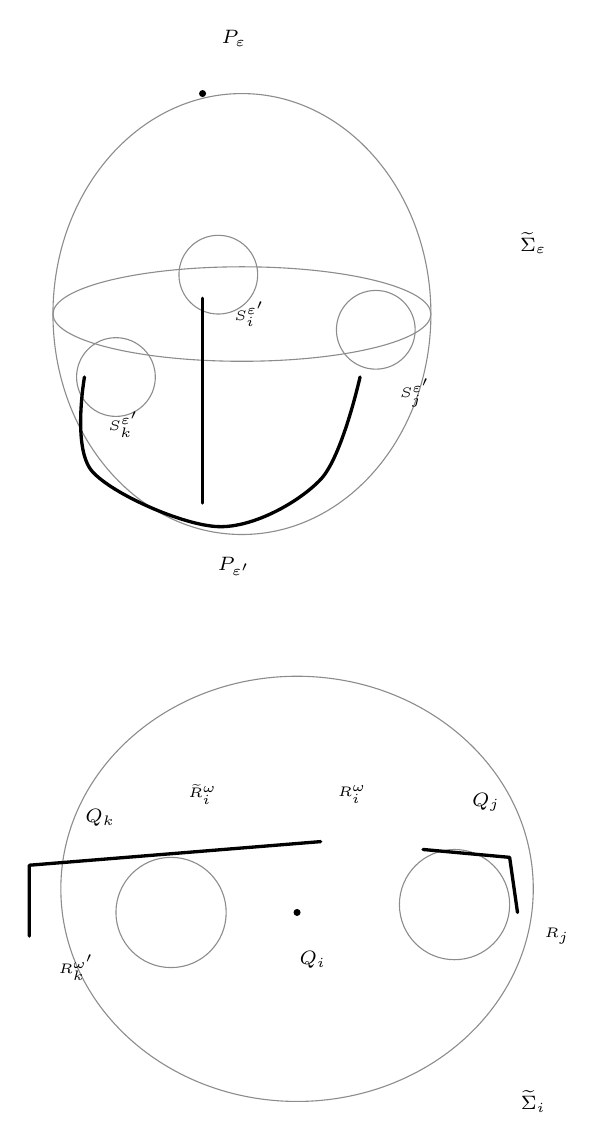
\begin{tikzpicture}[x=1mm,y=1mm,line cap=round,line join=round,font=\scriptsize]
\draw[pencil] (48,-42) ellipse[x radius=24, y radius=28];
\draw[pencil] (48,-42) ellipse[x radius=24, y radius=6];
\node[pt] at (43,-14) {};
\draw[pencil] (32,-50) circle[radius=5];
\draw[pencil] (45,-37) circle[radius=5];
\draw[pencil] (65,-44) circle[radius=5];
\draw[very thick] plot[smooth, tension=0.55] coordinates {(28,-50) (29,-62) (45,-69) (58,-63) (63,-50)};
\draw[very thick] (43,-40) -- (43,-66);
\node[inner sep=1pt] at (47,-7) {\scriptsize $P_\varepsilon$};
\node[inner sep=1pt] at (33,-56) {\tiny $S_k^{\varepsilon'}$};
\node[inner sep=1pt] at (49,-42) {\tiny $S_i^{\varepsilon'}$};
\node[inner sep=1pt] at (70,-52) {\tiny $S_j^{\varepsilon'}$};
\node[inner sep=1pt] at (47,-74) {\scriptsize $P_{\varepsilon'}$};
\node[inner sep=1pt] at (85,-33) {\scriptsize $\widetilde\Sigma_\varepsilon$};
\draw[pencil] (55,-115) ellipse[x radius=30, y radius=27];
\draw[pencil] (39,-118) circle[radius=7];
\draw[pencil] (75,-117) circle[radius=7];
\draw[very thick] (21,-121) -- (21,-112) -- (58,-109);
\draw[very thick] (71,-110) -- (82,-111) -- (83,-118);
\node[pt] at (55,-118) {};
\node[inner sep=1pt] at (30,-106) {\scriptsize $Q_k$};
\node[inner sep=1pt] at (43,-103) {\tiny $\widetilde R_i^{\omega}$};
\node[inner sep=1pt] at (62,-103) {\tiny $R_i^{\omega}$};
\node[inner sep=1pt] at (79,-104) {\scriptsize $Q_j$};
\node[inner sep=1pt] at (57,-124) {\scriptsize $Q_i$};
\node[inner sep=1pt] at (27,-125) {\tiny $R_k^{\omega'}$};
\node[inner sep=1pt] at (88,-121) {\tiny $R_j$};
\node[inner sep=1pt] at (85,-142) {\scriptsize $\widetilde\Sigma_i$};
\end{tikzpicture}
\end{document}
